\section{Alloy and Bounded Verification}
\label{sec:alloy}

The tool used in our approach is Alloy, a declarative modeling language combining first-order logic with relational calculus and associated quantifiers and operators, along with transitive closure.  It offers rich data modeling features based on class-like structures and an automatic form of analysis that is performed within a bounded scope using a SAT solver.  For \emph{simulation}, the analyzer can be directed to look for instances satisfying a property of interest.  For \emph{checking}, it looks for an instance violating an assertion: a counterexample.  The approach is \emph{scope complete} in the sense that all cases are checked within user-specified bounds.  Alloy's logic supports three distinct styles of expression, that of predicate calculus, navigation expressions, and relational calculus.  The language used for modeling is also used for specifying properties of interest and assertions.  Alloy supports expressions with integer values and basic arithmetic operations.

Alloy cannot check all possible cases, but instead relies on the small-scope hypothesis, refer to \figurename~\ref{pic:small}.

\begin{figure}
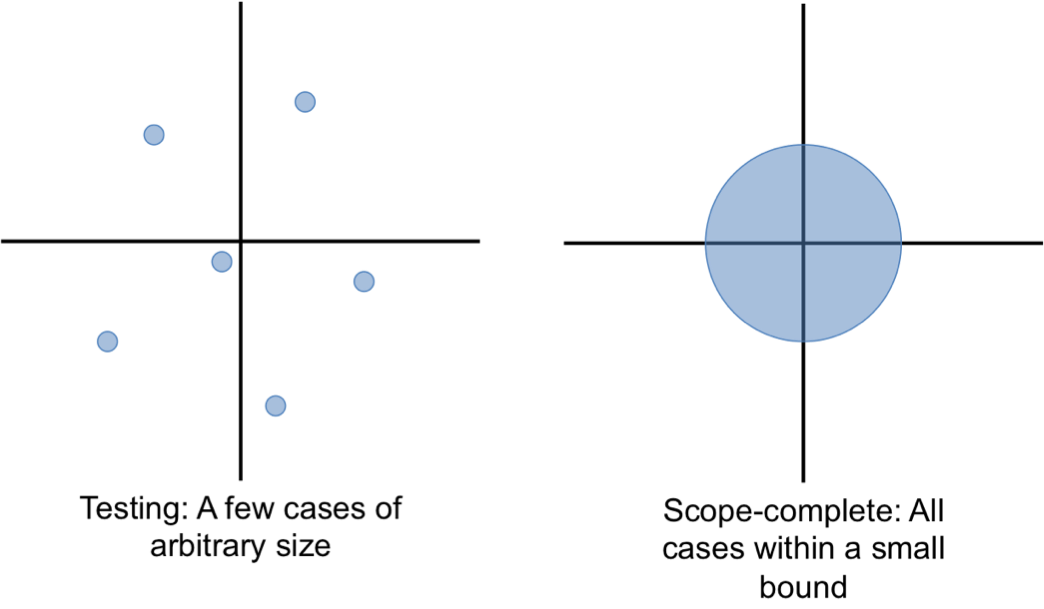
\includegraphics[width=\columnwidth]{images/smallscope}
\caption{Illustration of Small Scope Hypothesis (cite)}
\label{pic:small}
\end{figure}

Implicitness in specification; Alloy generates what might be viewed as input or data for operations.  This means, e.g., arbitrary sparse matrices are generated; contrast this with unit testing in which inputs must be created manually.  For numerical software, it is hard to perform `parts' of a large-scale simulation by simply extracting code... have to create `valid' data for input, populate data structures.  In alloy we describe properties required of data and Alloy generates it for us, so in some ways this is easier than testing a component of a large-scale program.

Proof obligations: mathematical formula to be proven in order to ensure that a component is correct.